\documentclass{article}
\usepackage{amsmath}
\usepackage{hyperref}
\usepackage[capitalise]{cleveref}
\usepackage[UKenglish]{babel}
\usepackage[UKenglish]{isodate}
\usepackage[utf8]{inputenc}
\usepackage[affil-it]{authblk}
\usepackage{amsfonts}
\usepackage{complexity}
\usepackage{fullpage}
\usepackage{listings}
\usepackage{mathrsfs}
\usepackage{pdfpages}
\usepackage{siunitx}
\usepackage{subcaption}
\usepackage{tikz}

\makeatletter
\DeclareRobustCommand{\crefnosort}[1]{%
  \begingroup\@cref@sortfalse\cref{#1}\endgroup
}
\makeatother

\usetikzlibrary{arrows}
\usetikzlibrary{arrows.meta}
\usetikzlibrary{calc}
\usetikzlibrary{positioning}
\usetikzlibrary{shapes}

\title{Probabilistic Inference via Weighted Model Counting: Algorithms,
  Encodings, and Random Instances}
\author{Paulius Dilkas \\[1ex] {\small Supervisors: Dr Vaishak Belle and Dr Ron
    Petrick}}
\affil{School of Informatics, University of Edinburgh}

\definecolor{first}{HTML}{1b9e77}
\definecolor{second}{HTML}{d95f02}
\definecolor{third}{HTML}{7570b3}
\definecolor{fourth}{HTML}{e7298a}
\definecolor{fifth}{HTML}{66a61e}

\begin{document}
\maketitle

\section{Introduction}

\begin{figure}
  \centering
  \begin{subfigure}{0.59\textwidth}
    \centering
    \begin{lstlisting}[escapeinside={(*}{*)}]
random Boolean Burglary (*$\sim$*) BooleanDistrib(0.001);
random Boolean Earthquake (*$\sim$*) BooleanDistrib(0.002);
random Boolean Alarm (*$\sim$*)
  if Burglary then
    if Earthquake then BooleanDistrib(0.95)
    else BooleanDistrib(0.94)
  else
    if Earthquake then BooleanDistrib(0.29)
    else BooleanDistrib(0.001);
random Boolean JohnCalls (*$\sim$*)
  if Alarm then BooleanDistrib(0.9)
  else BooleanDistrib(0.05);
random Boolean MaryCalls (*$\sim$*)
  if Alarm then BooleanDistrib(0.7)
  else BooleanDistrib(0.01);
    \end{lstlisting}
    \caption{BLOG}
    \label{fig:blog}
  \end{subfigure}
  \begin{subfigure}{0.40\textwidth}
    \centering
    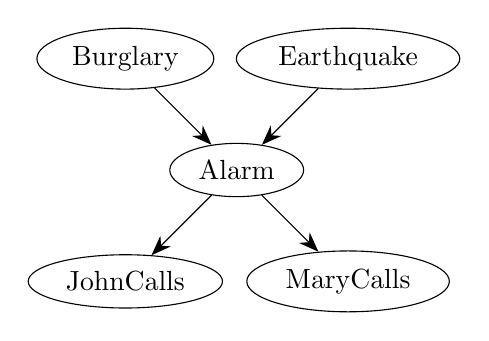
\begin{tikzpicture}[node distance=2cm]
      \node[draw,ellipse] (alarm) {Alarm};
      \node[draw,ellipse,above left of=alarm] (burglary) {Burglary};
      \node[draw,ellipse,above right of=alarm] (earthquake) {Earthquake};
      \node[draw,ellipse,below left of=alarm] (johnCalls) {JohnCalls};
      \node[draw,ellipse,below right of=alarm] (maryCalls) {MaryCalls};
      \draw[-{Stealth[scale=1.5]}] (burglary) -- (alarm);
      \draw[-{Stealth[scale=1.5]}] (earthquake) -- (alarm);
      \draw[-{Stealth[scale=1.5]}] (alarm) -- (johnCalls);
      \draw[-{Stealth[scale=1.5]}] (alarm) -- (maryCalls);
    \end{tikzpicture}
    \caption{Bayesian network}
    \label{fig:bn}
  \end{subfigure}
  \begin{subfigure}{0.59\textwidth}
    \centering
    \begin{lstlisting}
0.001 :: burglary.
0.002 :: earthquake.
0.95 :: alarm :- burglary, earthquake.
0.94 :: alarm :- burglary, \+ earthquake.
0.29 :: alarm :- \+ burglary, earthquake.
0.001 :: alarm :- \+ burglary, \+ earthquake.
0.9 :: johnCalls :- alarm.
0.05 :: johnCalls :- \+ alarm.
0.7 :: maryCalls :- alarm.
0.01 :: maryCalls :- \+ alarm.
    \end{lstlisting}
    \caption{ProbLog}
    \label{fig:problog}
  \end{subfigure}
  \begin{subfigure}{0.40\textwidth}
    \centering
    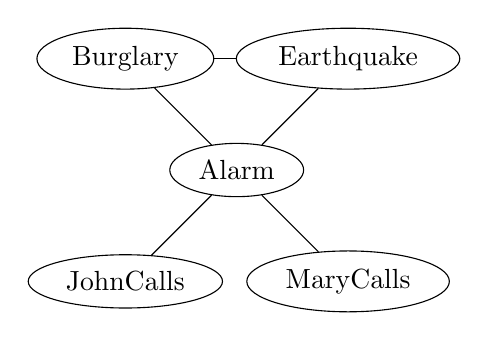
\begin{tikzpicture}[node distance=2cm]
      \node[draw,ellipse] (alarm) {Alarm};
      \node[draw,ellipse,above left of=alarm] (burglary) {Burglary};
      \node[draw,ellipse,above right of=alarm] (earthquake) {Earthquake};
      \node[draw,ellipse,below left of=alarm] (johnCalls) {JohnCalls};
      \node[draw,ellipse,below right of=alarm] (maryCalls) {MaryCalls};
      \draw (burglary) -- (earthquake);
      \draw (burglary) -- (alarm);
      \draw (earthquake) -- (alarm);
      \draw (alarm) -- (johnCalls);
      \draw (alarm) -- (maryCalls);
    \end{tikzpicture}
    \caption{Markov random field}
    \label{fig:mrf}
  \end{subfigure}
  \caption{Selected representations of an example probability distribution}
  \label{fig:representations}
\end{figure}

Probabilities, various representations of probability distributions, and the
computational problem known as probabilistic inference affect many fields
including life sciences, natural language processing, and robotics.
Probabilistic models have been used to analyse genetic
\cite{DBLP:journals/nar/MaeyerWRRM15,DBLP:journals/jcb/SakhanenkoG12} and
medical \cite{DBLP:conf/iaai/NatarajanKIJC13} data and in particular have been
successfully applied to breast cancer diagnosis and decision support
\cite{DBLP:conf/ilp/Corte-RealD017,DBLP:conf/pkdd/NassifKBPSC13}. In natural
language processing, probabilistic models have been used to extract events
\cite{DBLP:conf/emnlp/VenugopalCGN14} and knowledge
\cite{DBLP:conf/naacl/PoonV10} from text, classify sentences
\cite{DBLP:conf/emnlp/VerbekeAMFDR12}, efficiently model a language
\cite{DBLP:conf/icml/JerniteRS15}, solve textbook probability problems
\cite{DBLP:conf/ijcai/DriesKDBR17}, and form beliefs from reading various web
pages \cite{DBLP:conf/aaai/CarlsonBKSHM10}. Applications in robotics include
modelling object affordances
\cite{DBLP:conf/icra/MoldovanMOSR12,DBLP:conf/iros/MoldovanR14,DBLP:conf/ilp/MoldovanORMS11},
enabling a robot control system to deal with ambiguities in natural language
instructions \cite{DBLP:journals/ras/BeetzJMT10}, or more generally as the
robot's probabilistic knowledge representation system
\cite{DBLP:conf/icra/JainMB09}. Finally, these models have also been used for
many other tasks such as planning under uncertainty
\cite{DBLP:journals/jair/BoutilierDH99}, knowledge base construction
\cite{DBLP:journals/ijswis/NiuZRS12}, stream mining
\cite{DBLP:conf/icdm/ChandraSKTA14}, predicting the remaining useful life of a
hardware component \cite{vlasselaer2012statistical}, recommendation systems
\cite{DBLP:journals/corr/YangKAGN16}, and criminal activity prediction
\cite{DBLP:conf/sdm/DelaneyFCWJ10}. Probabilities (more specifically, transition
probabilities) are also central to Markov decision processes
\cite{bellman1957markovian} and partially observable Markov decision processes
\cite{aastrom1965optimal}, and so are heavily used in planning languages such as
relational dynamic influence diagram language (RDDL) \cite{sanner2010relational}
and probabilistic model checkers such as PRISM
\cite{DBLP:conf/cav/KwiatkowskaNP11}. Finally, probabilities are even used in
databases as a way to represent uncertainty about the correctness or accuracy of
data \cite{DBLP:series/synthesis/2011Suciu}.

Perhaps the best-known representations of probability distributions are
probabilistic graphical models (PGMs), i.e., graphs with vertices that
correspond to random variables. The graph can either be directed (as in Bayesian
networks \cite{DBLP:books/daglib/0066829}, see \cref{fig:bn}) or undirected (as
in Markov random fields \cite{spitzer1971markov}, see \cref{fig:mrf}). Both
Bayesian networks and Markov random fields have been extended to support
additional structure: relational Bayesian networks \cite{DBLP:conf/uai/Jaeger97}
can compactly describe a probability distribution over a relational structure,
and Markov logic networks (MLNs) \cite{DBLP:journals/ml/RichardsonD06} extend
Markov random fields with support for first-order logic. More examples of both
relational and first-order probabilistic models can be found in the survey paper
by de Salvo Braz et al. \cite{DBLP:series/sci/BrazAR08} or the book by De Raedt
et al. \cite{DBLP:series/synthesis/2016Raedt}.

Augmenting a programming language with probabilities is another common approach
to conveniently and compactly represent a probability distribution. Logic
programming languages, in particular, have been frequently used for this
purpose, examples of which include earlier languages such as independent choice
logic \cite{DBLP:journals/ai/Poole97} and PRISM \cite{DBLP:conf/ijcai/SatoK97}
as well as more recent ones such as ProbLog \cite{DBLP:conf/ijcai/RaedtKT07}
(see \cref{fig:problog}) and CP-logic \cite{DBLP:journals/tplp/VennekensDB09}.
Functional and imperative programming languages have also seen some use.
Probabilistic semantics in these languages typically rely on two constructs: the
ability to draw random values from probability distributions and the ability to
condition a program on observations \cite{DBLP:conf/icse/GordonHNR14}. Examples
of such languages include functional languages such as Church
\cite{DBLP:conf/uai/GoodmanMRBT08} and imperative languages like BLOG
\cite{DBLP:conf/ijcai/MilchMRSOK05} (see \cref{fig:blog}).

% Given a propositional formula, SAT asks whether there is a satisfying assignment
% of true or false values to variables such that the formula is satisfied. Model
% counting asks to count the number of such assignments. 

Weighted model counting (WMC) has emerged as the core computational problem
that can perform probabilistic inference for a variety of models. WMC
\cite{DBLP:journals/ai/ChaviraD08} is a generalisation of model counting that
assigns weights to literals and asks for the sum of the weights of all models
(i.e., satisfying assignments), where the weight of a model is equal to the
product of the weights of its literals. While propositional satisfiability (SAT)
is well-known as the prototypical and widely-researched NP-complete problem,
model counting has also been the focus of many algorithmic developments such as
heuristics and component caching \cite{DBLP:conf/ijcai/SharmaRSM19} and has a
wide range of applications including automatically synthesizing search
algorithms \cite{DBLP:journals/corr/abs-2009-10877}, assessing the quality of an
explanation of a machine learning model \cite{DBLP:conf/sat/NarodytskaSMIM19},
and analysing software for vulnerabilities
\cite{DBLP:conf/sp/ZhouQRZ18}.\footnote{Moreover, an annual model counting
  competition and workshop started running just last year
  (\url{https://mccompetition.org/}).} The two main variations/extensions of
model counting are projected model counting {\cite{DBLP:conf/sat/AzizCMS15} and
  WMC \cite{DBLP:journals/ai/ChaviraD08}.

The first (and most well-researched)
application of WMC is Bayesian network probabilistic inference
\cite{DBLP:conf/ecai/BartKLM16,DBLP:conf/ijcai/ChaviraD05,DBLP:conf/sat/ChaviraD06,DBLP:conf/kr/Darwiche02,DBLP:conf/aaai/SangBK05}.
Initially, this approach was motivated by context-specific independence
\cite{DBLP:conf/uai/BoutilierFGK96}, i.e., repeating probabilities in a
conditional probability table, and the difficulty in exploiting this redundancy
using previous probabilistic inference algorithms
\cite{DBLP:conf/kr/Darwiche02}. Other applications of WMC include probabilistic
logic programming language ProbLog
\cite{DBLP:journals/tplp/FierensBRSGTJR15,DBLP:conf/aaai/VlasselaerKDMR16},
probabilistic functional programming language Dice
\cite{DBLP:journals/pacmpl/HoltzenBM20}, and deep neural networks
\cite{DBLP:journals/corr/abs-2010-11926,DBLP:conf/icml/XuZFLB18}. WMC has been
extended to support continuous variables \cite{DBLP:conf/ijcai/BellePB15},
first-order logical formulas
\cite{DBLP:conf/ijcai/BroeckTMDR11,DBLP:journals/cacm/GogateD16}, and infinite
domains \cite{DBLP:conf/aaai/Belle17}. It was also observed that replacing real
numbers with addition and multiplication with an arbitrary commutative semiring
allows WMC to subsume a variety of other problems such as most probable
explanation, shortest path, and calculating gradients
\cite{DBLP:journals/ijar/BelleR20,DBLP:journals/japll/KimmigBR17}.

Despite the variety of representations, probabilistic inference (via WMC and
otherwise, more on this in the next section) can be seen as a single
computational problem. Thus, it is all the more important to develop WMC
algorithms with good empirical performance, understand the comparative strengths
and weaknesses of different approaches, and optimise the encoding process that
transforms the initial representation of a probability distribution to a
representation accepted by the algorithm. In my work, I address this problem by
assessing the empirical performance of these algorithms on random instances of
different kinds, revealing the weaknesses of the standard definition of WMC, and
suggesting more expressive alternatives.

This document has four sections and four appendices:
\begin{itemize}
\item \Cref{sec:background} provides some background on probabilistic inference
  algorithms, WMC algorithms, and knowledge compilation.
\item \Cref{sec:progress} describes the research progress made this academic
  year.
\item \Cref{sec:future} provides a plan for the rest of my degree.
\item \crefnosort{app:cp,app:uai,app:sat} contain papers published since last
  year's review.
\item And last year's review itself is included in \cref{app:previous}.
\end{itemize}

\section{Background on Algorithms} \label{sec:background}

The problem of computing some probability from a given representation of a
probability distribution can be seen as a version of a more general problem
known as SumProd
\cite{DBLP:journals/jair/BacchusDP09,DBLP:journals/ai/Dechter99}. It is
characterised by a set of discrete variables and a set of functions from some
subsets of the variables to a commutative semiring. SumProd then asks to compute
the sum over all values of all variables of the product of all functions. Many
problems such as SAT, constraint satisfaction and optimisation, model counting,
and most probable explanation can be described as variations of SumProd
\cite{DBLP:journals/jair/BacchusDP09,DBLP:journals/ai/Dechter99}. It is often
convenient to consider two graphs associated with each instance of SumProd. Its
canonical hypergraph has variables as vertices and function domains as edges,
and its primal graph (also known as the Gaifman graph and by many other names)
is the simple graph with variables as vertices and an edge between two variables
if there is a function that depends on both of them.

Many algorithms for probabilistic inference have been proposed. Variable
elimination \cite{DBLP:journals/ai/Dechter99} works by nondeterministically
choosing an ordering of variables and `summing out' each variable in the chosen
order. The well-known Davis-Putnam algorithm \cite{DBLP:journals/jacm/DavisP60}
for SAT is an example of variable elimination
\cite{DBLP:journals/jair/BacchusDP09}. Recursive conditioning
\cite{DBLP:journals/ai/Darwiche01} is a divide-and-conquer algorithm that relies
on a branch decomposition of the hypergraph to initialise variables in such a
way to split the problem into multiple smaller problems that can be solved
independently. AND/OR search
\cite{DBLP:journals/ai/DechterM07,nilsson1980principles} is a similar technique
that utilises pseudo trees of the primal graph instead of branch decompositions.
Belief propagation (also known as message passing) \cite{DBLP:conf/aaai/Pearl82}
is an approximation algorithm that converges to the exact answer when the primal
graph is a tree, and join (or junction) tree algorithm \cite{lauritzen1988local}
extends belief propagation to arbitrary primal graphs via tree decompositions.

\subsection{WMC}

\begin{figure}
  \centering
  \begin{subfigure}{0.30\textwidth}
    \centering
    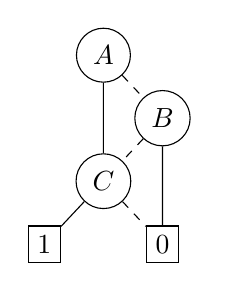
\begin{tikzpicture}[level distance=0.8cm]
      \node[draw,circle] (A) {$A$}
      child {edge from parent[draw=none]}
      child {node[draw,circle] (B) {$B$} edge from parent[dashed]
        child {node[draw,circle,solid] (C) {$C$} edge from parent[dashed]
          child {node[draw,rectangle,solid] {$1$} edge from parent[solid]}
          child {node[draw,rectangle,solid] (0) {$0$}}
        }
        child {edge from parent[draw=none]}
      };
      \draw (A) -- (C);
      \draw (B) -- (0);
    \end{tikzpicture}
    \caption{(RO)BDD}
  \end{subfigure}
  \begin{subfigure}{0.30\textwidth}
    \centering
    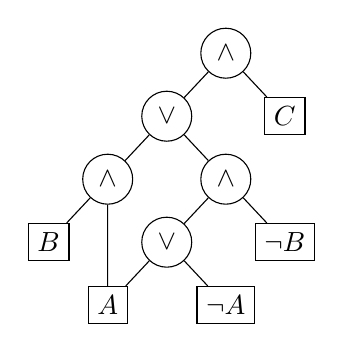
\begin{tikzpicture}[level distance=0.8cm]
      \node[draw,circle] {$\land$}
      child {node[draw,circle] {$\lor$}
        child {node[draw,circle] (parent) {$\land$}
          child {node[draw,rectangle] {$B$}}
          child {edge from parent[draw=none]}
        }
        child {node[draw,circle] {$\land$}
          child {node[draw,circle] {$\lor$}
            child {node[draw,rectangle] (A) {$A$}}
            child {node[draw,rectangle] {$\neg A$}}
          }
          child {node[draw,rectangle] {$\neg B$}}
        }
      }
      child {node[draw,rectangle] {$C$}};
      \draw (parent) -- (A);
    \end{tikzpicture}
    \caption{d-DNNF}
  \end{subfigure}
  \begin{subfigure}{0.30\textwidth}
    \centering
    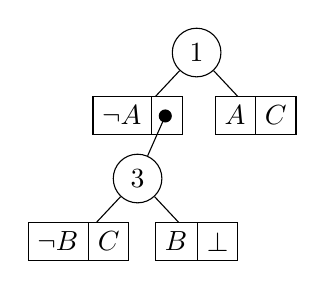
\begin{tikzpicture}[level distance=0.8cm]
      \tikzset{
        mysplit/.style={
          draw,
          rectangle,
          rectangle split,
          rectangle split horizontal,
          rectangle split parts=2
        }
      }
      \node[draw,circle] {$1$}
      child {node[mysplit] (bullet) {
          \nodepart{one} $\neg A$
          \nodepart{two}
        }
        child {node[draw,circle] (3) {$3$} edge from parent[draw=none]
          child {node[mysplit] {
              \nodepart{one} $\neg B$
              \nodepart{two} $C$
            }
          }
          child {node[mysplit] {
              \nodepart{one} $B$
              \nodepart{two} $\bot$
            }
          }
        }
      }
      child {node[mysplit] {
          \nodepart{one} $A$
          \nodepart{two} $C$
        }};
      \draw[*-] let \p1 = (bullet.two), \p2 = (bullet.center) in ({\x1 + 2.5},{\y2 + 2}) -- (3);
    \end{tikzpicture}
    \caption{SDD}
  \end{subfigure}
  \caption{Example diagrams for $C \land (A \lor \neg B)$}
  \label{fig:kc}
\end{figure}

Many WMC algorithms rely on knowledge compilation, i.e., compilation of the
structure of the initial representation into a form that allows one to perform
various operations and answer queries of interest in time polynomial in the size
of the compiled representation. Traditionally, the initial representation is a
propositional formula. Many such representations have been proposed
\cite{DBLP:journals/jair/DarwicheM02}. Amongst them, the ones that are used in
probabilistic inference include (reduced ordered) binary decision diagrams
((RO)BDDs) \cite{DBLP:journals/tc/Bryant86}, deterministic decomposable negation
normal form (d-DNNF) \cite{DBLP:journals/jancl/Darwiche01}, sentential decision
diagrams (SDDs) \cite{DBLP:conf/ijcai/Darwiche11}, and probabilistic SDDs
\cite{DBLP:conf/kr/KisaBCD14}---some of them are pictured in \cref{fig:kc}. A
BDD is similar to a decision tree that ends with either one or zero but
generalised to a directed acyclic graph. Both d-DNNF and SDD are normal forms
for propositional formulae that satisfy certain properties. Probabilistic SDDs
extend SDDs with probability labels on edges. BDDs are a strict subset of SDDs
that are a strict subset of d-DNNF \cite{DBLP:conf/ijcai/Darwiche11}.

WMC algorithms can be classified as those based on search, knowledge
compilation, or algebraic decision diagrams (ADDs). The only search-based WMC
algorithm is Cachet
\cite{DBLP:conf/sat/SangBBKP04,DBLP:conf/sat/SangBK05,DBLP:conf/aaai/SangBK05}
which extends the SAT solver ZChaff
\cite{DBLP:conf/dac/MoskewiczMZZM01,DBLP:conf/iccad/ZhangMMM01}. WMC algorithms
based on knowledge compilation include c2d \cite{DBLP:conf/ecai/Darwiche04} and
d4 \cite{DBLP:conf/ijcai/LagniezM17} that compile to d-DNNF and miniC2D
\cite{DBLP:conf/ijcai/OztokD15} that compiles to SDDs. Other approaches to WMC
include approximate \cite{DBLP:conf/aaai/RenkensKBR14} and parallel algorithms
\cite{DBLP:conf/pgm/DalLL18,DBLP:conf/esa/FichteHWZ18}, quantum computing
\cite{DBLP:conf/ecai/Riguzzi20} and reduction to model counting
\cite{DBLP:conf/ijcai/ChakrabortyFMV15}.

Similarly to how BDDs represent Boolean functions, ADDs represent pseudo-Boolean
functions, i.e., while (non-trivial) BDDs always have two sinks marked with one
and zero, ADDs can have any number of sinks that contain, typically, real
numbers \cite{DBLP:journals/fmsd/BaharFGHMPS97}. ADDs have been extended to
represent the additive and multiplicative structure in sink values more
compactly \cite{DBLP:conf/ijcai/SannerM05} and to support first-order logic
\cite{DBLP:journals/ai/SannerB09} and continuous variables
\cite{DBLP:conf/uai/SannerDB11}. ADDs have been used to represent MDP value
functions \cite{DBLP:conf/uai/HoeySHB99} and probabilities in PGMs
\cite{DBLP:conf/ijcai/ChaviraD07,DBLP:conf/uai/GogateD11}. The two WMC
algorithms based on ADDs are ADDMC \cite{DBLP:conf/aaai/DudekPV20} and DPMC
\cite{DBLP:conf/cp/DudekPV20}. The main difference between them is that ADDMC
relies on heuristics to plan the order of operations whereas DPMC uses a tree
decomposition instead.

\section{Progress To Date} \label{sec:progress}

\begin{figure}[t]
  \centering
  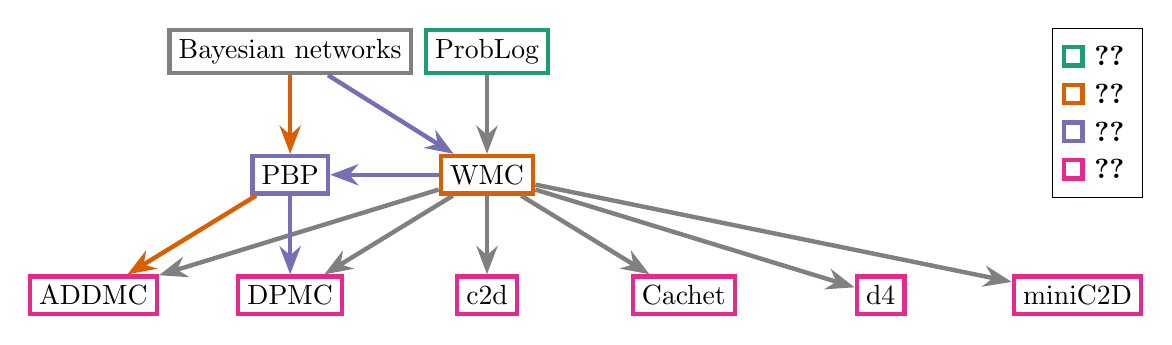
\begin{tikzpicture}[node distance=2.5cm]
    \node[draw,ultra thick,color=gray,text=black] (bn) {Bayesian networks};
    \node[draw,ultra thick,right of=bn,color=first,text=black] (problog) {ProbLog};
    \node[draw,ultra thick,below=1cm of bn,color=third,text=black] (pbp) {PBP};
    \node[draw,ultra thick,below=1cm of problog,color=second,text=black] (wmc) {WMC};
    \node[draw,ultra thick,below=1cm of pbp,color=fourth,text=black] (dpmc) {DPMC};
    \node[draw,ultra thick,color=fourth,text=black,left of=dpmc] (addmc) {ADDMC};
    \node[draw,ultra thick,right of=dpmc,color=fourth,text=black] (c2d) {c2d};
    \node[draw,ultra thick,right of=c2d,color=fourth,text=black] (cachet) {Cachet};
    \node[draw,ultra thick,right of=cachet,color=fourth,text=black] (d4) {d4};
    \node[draw,ultra thick,right of=d4,color=fourth,text=black] (minic2d) {miniC2D};
    \draw[-{Stealth},ultra thick,color=third] (bn) -- (wmc);
    \draw[-{Stealth},ultra thick,color=second] (bn) -- (pbp);
    \draw[-{Stealth},ultra thick,color=gray] (problog) -- (wmc);
    \draw[-{Stealth},ultra thick,color=third] (wmc) -- (pbp);
    \draw[-{Stealth},ultra thick,color=gray] (wmc) -- (addmc);
    \draw[-{Stealth},ultra thick,color=gray] (wmc) -- (dpmc);
    \draw[-{Stealth},ultra thick,color=gray] (wmc) -- (c2d);
    \draw[-{Stealth},ultra thick,color=gray] (wmc) -- (cachet);
    \draw[-{Stealth},ultra thick,color=gray] (wmc) -- (d4);
    \draw[-{Stealth},ultra thick,color=gray] (wmc) -- (minic2d);
    \draw[-{Stealth},ultra thick,color=second] (pbp) -- (addmc);
    \draw[-{Stealth},ultra thick,color=third] (pbp) -- (dpmc);
    \matrix[draw,below left] at (current bounding box.north east) {
      \node[draw,color=first,ultra thick,label=right:\cref{app:cp}] {}; \\
      \node[draw,color=second,ultra thick,label=right:\cref{app:uai}] {}; \\
      \node[draw,color=third,ultra thick,label=right:\cref{app:sat}] {}; \\
      \node[draw,color=fourth,ultra thick,label=right:\cref{sec:future}] {}; \\
    };
  \end{tikzpicture}
  \caption{Outline of concepts relevant to my past and future work. The first
    row contains representations of probability distributions that are and have
    been relevant to my work. The second row contains encodings, i.e.,
    computational problems that encode probabilistic inference. The third row
    contains WMC algorithms. Gray arrows and boxes denote connections and
    concepts that are already known from previous work, and I have not worked
    on. A coloured arrow or box indicates that my work relates to that concept
    or interaction of concepts, and the colour coding describes which past or
    future paper the concept is related to.}
  \label{fig:overview}
\end{figure}

In this section, the progress made throughout this academic year is described
according to the work plan from my first-year review.\footnote{The first-year
review (with its appendices) is included as \cref{app:previous}.} The reader
is advised to refer to \cref{fig:overview} as a guide for how my previous and
future research projects relate to one another. The acronym PBP will be
explained shortly.

\begin{description}
\item[WP 1] (`On the Equivalence of Constants in Relational Knowledge
  Bases'---the paper that attempted to characterise how logic programs can act
  as morphisms and describe the necessary conditions on domains and codomains)
  was abandoned. While trying to consider reviewer feedback as well as update
  and strengthen the paper, I found an important ambiguity: when defining what
  constants are `captured' and `transferred' by a clause, I fail to specify
  whether each argument is a  constant or a variable. In the
  former case, that makes the main theorem of the paper completely trivial.
  Whereas in the latter case, the theorem becomes incorrect. I spent several
  weeks looking for ways to transform the paper into something both correct and
  valuable. The best idea I could find was to use the perspective from this
  paper in the context of inductive logic programming (ILP). However, this line
  of research seemed unpromising: since ILP is a fairly mature field
  \cite{DBLP:conf/ijcai/CropperDM20}, it is unlikely that a naive foundational
  approach can be competitive with the state of the art.
\item[WP 2] (`Generating Random Logic Programs Using Constraint
  Programming'---the paper that develops a constraint model for (probabilistic)
  logic programs with support for arbitrary formulas in clause bodies and some
  custom constraints with propagation and entailment algorithms) was revised to
  include an experimental comparison of ProbLog inference algorithms and
  published and presented at CP~2020 (i.e., the premier conference for
  constraint programming).\footnote{See \cref{app:cp} for the camera-ready
    version.} I also gave three more talks about it:
  \begin{itemize}
  \item at the local AIAI seminar,
  \item for the Formal Analysis, Theory and Algorithms research section at the
    University of Glasgow,
  \item and at the FMAI~2021 workshop.
  \end{itemize}
\item[WP 3] (`Weighted Model Counting with Conditional Weights for Bayesian
  Networks'---the paper that develops a more succinct WMC-like encoding for
  Bayesian network probabilistic inference) was completed in full, although the
  emphasis shifted more towards experimental results than theory. It was first
  (unsuccessfully) submitted to AAAI~2021. Based on reviewer feedback, I updated
  the experimental section to compare not just various encodings with the same
  algorithm but also all of the encodings with the algorithms used in the
  original papers. The updated version was published at UAI~2021 and can be
  found in \cref{app:uai}. I was also invited to the program committee for this
  conference.
  \item[WP 4] (`Abstractions as Homomorphisms'---an algebraic perspective on
  abstraction) was abandoned due to a lack of contributions that could be made.
  Indeed, any contribution would have to be theoretical, empirical, or
  interpretability-related. Significant theoretical contributions are unlikely
  because the theory of abstractions has already been explored before without
  leaving behind any big unanswered questions \cite{DBLP:journals/kbs/Belle20}.
  While previous work could be rephrased more simply and extended with more
  detail, the contributions would still be marginal.

  Furthermore, considering abstractions at their full level of generality is
  unlikely to be a viable method for improving inference speed because any
  abstraction is likely to be more computationally expensive than inference.
  Moreover, previous work on preprocessing for WMC left the field in an
  uncomfortable situation: preprocessing techniques for WMC were identified and
  described in a paper \cite{DBLP:conf/aaai/LagniezM14} whose main focus is on
  model counting, and the closed-source implementation of those techniques is
  unsuitable for WMC.

  Finally, a substantial issue with considering abstraction as a tool for
  interpretability---especially in the context of probabilistic relational
  models---is that the low-level building blocks such as predicate and constant
  names are usually semantically meaningful. Thus, replacing such a model with a
  simpler alternative that instead uses high-level concepts that are unlikely to
  correspond to words in any natural language is unlikely to improve
  interpretability despite the potential simplicity of this type of abstraction.
\item
  Furthermore, a new paper (not covered in the previous annual report) was
  written and published at SAT~2021 (see \cref{app:sat}). It originated as an
  attempt to improve \textbf{WP 3}: while the experimental results were
  impressive in the initial version of the paper, adding other algorithms
  revealed that instead of improving the state of the art by two orders of
  magnitude as originally thought, the suggested encoding was only fixing an
  underperforming algorithm and making its performance in line with other
  algorithms.

  The algorithm used for these experiments (ADDMC) was published
  only last year \cite{DBLP:conf/aaai/DudekPV20} and its experimental study
  includes some of the data used in my experiments as well as some new
  instances---one has to wonder whether the latter were added to improve the
  algorithm's comparative performance. Unlike most other WMC algorithms, ADDMC
  does not perform knowledge compilation. Instead, it gradually builds and
  simplifies an ADD, which eventually only contains the answer probability.

  First, my new paper replaces the previously used algorithm with its even newer
  version DPMC \cite{DBLP:conf/cp/DudekPV20}. The main improvement over ADDMC
  comes from the use of approximately-minimal-treewidth tree decompositions
  instead of heuristics for planning the order of operations. After checking
  that DPMC performs very similarly with all encodings (including my own) and
  similarly to other WMC algorithms, the need to shift the contribution of my
  paper elsewhere became apparent.

  The main advantage of the encoding I proposed earlier was that it avoided
  parameter variables---something I claimed is completely unnecessary at
  least in WMC algorithms based on ADDs. However, the encoding was particularly
  rigid in that it always compiled each conditional probability table (CPT) in a
  Bayesian network into an ADD before doing anything else. Although this
  resulted in great inference speed improvements on some instances, e.g., when
  most of the probabilities in a CPT are equal, there is no reason to believe
  that such an approach is always optimal. Being unable to suggest a new
  encoding that outperforms others, I decided to investigate how parameter
  variables could be removed from already-existing encodings. This led to a
  generalisation of WMC based on pseudo-Boolean functions that I named
  pseudo-Boolean projection (PBP). I then show how any WMC instance can be
  transformed into a PBP instance and identify conditions under which such a
  transformation can remove parameter variables. This transformation applies to
  four out of the five WMC encodings for Bayesian networks. Finally, experiments
  showed that (at least for some encodings) parameter variable removal can
  significantly improve inference speed and supersede the previous state of the
  art.
\end{description}

\section{Future Goals} \label{sec:future}

The experiments in my papers in \cref{app:uai,app:sat} as well as in previous
work by others \cite{DBLP:conf/aaai/DudekPV20,DBLP:conf/cp/DudekPV20}
demonstrate that the differences amongst WMC algorithms are poorly understood,
i.e., the algorithms perform very similarly overall, but with significant
differences on subsets of benchmark data. In other words, which algorithm is the
best depends entirely on what data it is run on, and we have no idea what
properties of a WMC instance make it more suitable for a search-based,
compilation-based, or ADD-based approach. Therefore, the paper I am working on
now aims to:
\begin{itemize}
\item Establish the parameterized complexity of DPMC, showing that it scales
  worse (than other algorithms) with respect to the treewidth of the primal
  graph of the input propositional formula in conjunctive normal form (CNF) (we
  call this primal treewidth).
\item Propose a new random model for CNF formulas that allows us to generate
  instances of varying primal treewidth and use it to experimentally show how
  the performance of WMC algorithms depends on various properties of the
  instance such as density, primal treewidth, and the proportion of literal
  weights that are particularly `simplifying', e.g., zero, one, and perhaps a
  half.
\end{itemize}
This should be enough material for a conference submission and enable me to
start writing my thesis with all the main chapters already in place. Time
permitting, I am going to explore the following extensions.
\begin{itemize}
\item The original set of experiments will only consider $k$-CNF instances, but
  can then be extended to include non-$k$-CNF as well (as this would more
  realistically represent real instances).
\item Preliminary experiments show that one of the algorithms (Cachet) performs
  much better on random instances than any other algorithm, even though it
  slightly underperforms on real data. It would be interesting to find a random
  model of CNF instances where that is no longer the case. One idea for this is
  to `obfuscate' the random instances in a way similar to the typical structure
  of a real instance, i.e., by introducing new variables that are defined to be
  equivalent to a conjunction of randomly selected literals.
\item Another potential improvement is to consider measuring arithmetic
  complexity (e.g., the number of addition and multiplication operations that
  are performed on the weights) instead of time and see if the relative
  performance of the algorithms stays the same or not. This would separate the
  quality of the solution from the time it takes to find it. Knowing whether an
  algorithm underperforms because it chooses a suboptimal solution or because it
  takes too long to find one would then help in creating even better algorithms.
\end{itemize}

\paragraph{Estimated duration:} 9 months. Note that the total estimated duration
for these projects leaves sufficient time for thesis writing and potential
unexpected delays in line with the plan from last year.

\paragraph{Risks and contingencies.} One risk that I have already encountered is
that having all of the following can lead to an infeasible amount of computation
time:
\begin{itemize}
\item a time limit that is both similar to the time limits used in other
  experimental studies and provides enough `space' for a growth curve to express
  itself,
\item enough different parameter values so that the plots look more like the
  beautiful and barely-pixelated plots of today (e.g.,
  \cite{DBLP:conf/cp/McCreeshPP19,DBLP:journals/jair/McCreeshPST18}) and less
  like my tiny experimental setup in \cref{app:cp},
\item enough different random instances for each combination of parameter values
  so that a reliable median can be observed despite high variance.
\end{itemize}
This risk has been addressed in two ways:
\begin{itemize}
\item The time limit was reduced to \SI{100}{\second} and could be reduced
  further (e.g., a similar paper uses only a \SI{10}{\second} time limit
  \cite{DBLP:conf/ijcai/DudekMV17}).
\item Instead of iterating over the values of all parameters in one big
  experiment, I split it into two smaller experiments where some variables are
  held constant and others are allowed to vary.
\end{itemize}
Another risk is that the experimental results may be unclear and/or not easily
explainable. However, as random WMC instance generation is a completely
unexplored area, so even weird or imperfect results would still count as
valuable and interesting. Moreover, any unexpected differences in the way the
algorithms perform on random and real data can always be likened to the
equivalent situation with SAT algorithms.

\bibliographystyle{acm}
\bibliography{report}

\includepdf[pages=-,pagecommand=\thispagestyle{plain},picturecommand*={%
  \put(70,750){%
    \parbox{\textwidth}{\pagenumbering{gobble}\appendix\section{Published Paper (CP 2020)}\label{app:cp}}
  }}]{../../published/random-logic-programs/paper/paper.pdf}
\includepdf[pages=-,pagecommand=\thispagestyle{plain},picturecommand*={%
  \put(70,750){%
    \parbox{\textwidth}{\crefalias{section}{appendix}\section{Published Paper (UAI 2021)}\label{app:uai}}
  }}]{../../published/wmc-without-parameters/doc/UAI_paper/paper.pdf}
\includepdf[pages=-,pagecommand=\thispagestyle{plain},picturecommand*={%
  \put(70,750){%
    \parbox{\textwidth}{\crefalias{section}{appendix}\section{Published Paper (SAT 2021)}\label{app:sat}}
  }}]{../../published/wmc-without-parameters/doc/SAT_paper/paper.pdf}

\includepdf[pages=-,pagecommand=\thispagestyle{plain},picturecommand*={%
  \put(70,750){%
    \parbox{\textwidth}{\crefalias{section}{appendix}\section{First-Year Review}\label{app:previous}}
  }}]{../review1/review.pdf}

\end{document}